\documentclass{whutmod}
\usepackage[linesnumbered,ruled,lined]{algorithm2e}
\usepackage{amsmath,amsfonts,bm}
\usepackage{graphicx}
\usepackage{booktabs}
\usepackage{hyperref}
\usepackage{setspace}
\usepackage{natbib}
\usepackage{listings}
\bibliographystyle{unsrt}

% Team and member information
\team{10}
\membera{刘子川}
\joba{编程}
\memberb{程宇}
\jobb{建模}
\memberc{祁成}
\jobc{写作}

% Hyperlink setup
\hypersetup{
    colorlinks=true,
    linkcolor=black,
    citecolor=black
}

% Custom commands
\newcommand{\udots}{\mathinner{\mskip1mu\raise1pt\vbox{\kern7pt\hbox{.}}
        \mskip2mu\raise4pt\hbox{.}\mskip2mu\raise7pt\hbox{.}\mskip1mu}}
\newcommand{\upcite}[1]{\textsuperscript{\cite{#1}}}

% Title and problem number
\title{基于卷积自编码与k-medoids模型的指纹编码与分类}
\tihao{2}

\begin{document}
    \maketitle
    \thispagestyle{empty}

    % Abstract
    \begin{abstract}
        指纹识别系统的存储量巨大,提高指纹编码率具有重要意义。本文提出利用深度学习方法建立卷积自编码器模型,在非线性学习空间中有损压缩编码,并根据编码距离对指纹进行聚类。

        为消除指纹图像噪声和伪特征点影响,设计了预处理策略体系以统一图像尺度、细化纹线骨架。首先对指纹图像进行灰度值线性归一化处理,尺寸放缩后利用\textbf{分数阶微分算子}构造掩膜进行图像增强,最后通过方向场确定脊线实现像素二值化。预处理保留了指纹的连接状态、拓扑结构和纹理信息,剔除了次要纹线宽度信息,有利于后续编码。

        针对问题一,鉴于小样本条件下难以有效提取指纹特征的问题,设计了一种\textbf{卷积自编码网络}的特征提取算法。将预处理后的图像信号用\textbf{卷积核}转化到高维特征空间,利用大量无标签指纹样本训练卷积自编码器网络。通过损失函数\textbf{KL散度}进行\textbf{无监督学习},编码出最佳线性空间特征。训练提取的指纹特征损失率仅为\textbf{0.04\%},具有高还原度。

        针对问题二,对卷积自编码器生成的编码向量进行归一化处理,设计加权相似度量化指纹间相似性。计算归一化编码向量的\textbf{谷本系数}、\textbf{皮尔逊相关系数}和\textbf{马氏距离},同向化处理后加权求和,得到量化相似度。相似度热图可视化显示指纹间的异同。

        针对问题三,建立中心聚类模型,以问题二的量化相似度为代价函数,使用\textbf{k-medoids}算法选取聚类中心完成分类。对于附件中的16个指纹样本,基于加权相似度计算每对样本的相似度,选取$k$个样本点作为聚类中心,以样本到中心的平均相似度为代价函数。遍历聚类中心组合,当$k=4$时代价函数最优,分类结果为样本$\bm{10}$独立为一组,其余三组为$\bm{\{2,3,5\}}$、$\bm{\{1,4,7,11,16\}}$和$\bm{\{6,8,9,12,13,14,15\}}$。

        本文的优点为:1. 采用卷积核提取指纹细节,大幅降低数据维度的同时挖掘图像特征。2. 相较传统编码,模型具有较强的个体表征能力,可通过解码器高精度还原图像。

        \keywords{
            卷积自编码器 \quad
            分数阶微分算子 \quad
            k-medoids \quad
            无监督学习
        }
    \end{abstract}

    % Table of contents
    \thispagestyle{empty}
    \tableofcontents
    \setcounter{page}{0}
    \newpage

    % Problem restatement
    \section{问题重述}
        \subsection{问题背景}
            自动指纹识别系统(Automated Fingerprint Identification System, AFIS)在多个领域有广泛应用。研究主要集中在图像增强、指纹分类和细节匹配三个方面,分为“离线部分”和“在线部分”。如图~\ref{lssct}所示,离线部分包括采集指纹、提取细节点、存储到模板库;在线部分包括采集指纹、提取细节点并与模板库匹配,判断是否来自同一手指\upcite{1,3}。指纹分类用于大规模指纹库中减少搜索范围。指纹图像占用空间大,像素信息不适合计算机分析,需用最少字节描述指纹内在结构、形态和特征。AFIS可扫描犯罪现场指纹,与执法机关的指纹档案比对,列出匹配百分比供专家验证\upcite{2}\footnote{https://baike.baidu.com/item/AFIS/2851410?fr=aladdin}。

            \begin{figure}[H]
                \centering
                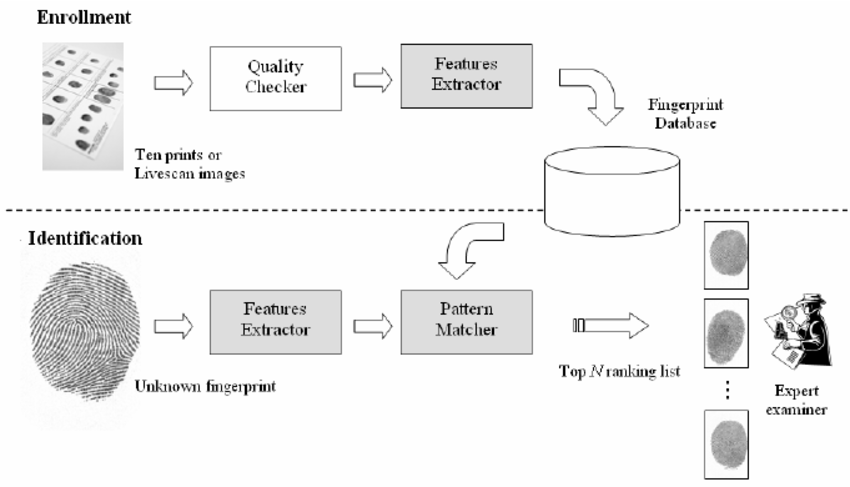
\includegraphics[width=.8\textwidth]{figures/AFIS.png}
                \caption{自动指纹识别系统框图}\label{lssct}
            \end{figure}

        \subsection{问题概述}
            围绕附件中的16幅指纹图像,不借助现有指纹软件,提出以下问题:

            \textbf{编码:} 给出一种用不超过200字节(称为“指纹密码”)描述指纹基本特征的表示方法,介绍其数学原理。

            \textbf{匹配:} 实现编码方法,为每幅指纹生成“指纹密码”。基于这些表示,比较指纹间的异同及相似程度。

            \textbf{应用:} 对比并归类16个指纹,给出依据和结果。

    % Model assumptions
    \section{模型假设}
        \begin{itemize}
            \item[(1)] 附件中所有指纹图像为清晰完整图像,无压缩信息损失。
            \item[(2)] 指纹图像特征具有代表性,包含正常人指纹的所有特征。
        \end{itemize}

    % Symbol description
    \section{符号说明}
        \begin{table}[H]
            \centering
            \setstretch{0.8}
            \setlength{\tabcolsep}{12mm}
            \begin{tabular}{cc}
                \toprule[1.5pt]
                \multicolumn{1}{m{5cm}}{\centering 符号} & \multicolumn{1}{m{5cm}}{\centering 说明} \\
                \midrule[1pt]
                $P_i$ & 第$i$张图像,$i \in \{1, 2, \dots, 16\}$ \\
                $u_{P(x,y)}$ & 像素矩阵 \\
                $(x,y)$ & 像素点位置值 \\
                $fringe_{x1}, fringe_{x2}$ & 图片的上下边界 \\
                $fringe_{y1}, fringe_{y2}$ & 图片的左右边界 \\
                $E$ & 信息熵 \\
                $iDir$ & 脊线方向 \\
                $\gamma$ & 编码器的图像编码 \\
                $b$ & 编码大小 \\
                $Z$ & 解码器还原的图像矩阵 \\
                $epoch$ & 迭代次数 \\
                $in/out$ & 出/入通道数 \\
                $lr$ & 学习率 \\
                $k_i$ & 卷积核$i$ \\
                $T$ & 谷本系数 \\
                $P$ & 皮尔逊相关系数 \\
                $M$ & 马氏距离 \\
                $\{c_i\}$ & 聚类中心 \\
                $\max_{1 \leqslant j \leqslant k} S(\gamma_i, c_j)$ & 样本点$\gamma_i$与$\{c_i\}$间的最高相似度值 \\
                \bottomrule[1.5pt]
            \end{tabular}
            \begin{tablenotes}
                \item 注:表中未说明的符号以首次出现处为准
            \end{tablenotes}
        \end{table}

    % Data preprocessing
    \section{数据预处理}
        在搭建模型前,对指纹图像进行预处理以统一规格、去除噪声,流程如图~\ref{dfsg}所示。

        \begin{figure}[H]
            \centering
            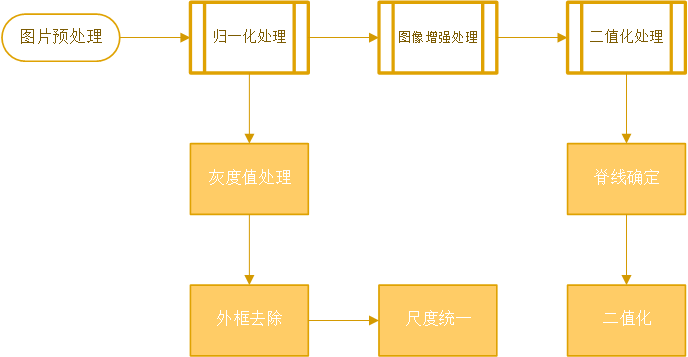
\includegraphics[width=.9\textwidth]{figures/chou4.png}
            \caption{图片数据预处理流程}\label{dfsg}
        \end{figure}

        \subsection{归一化处理}
            \subsubsection{灰度值处理}
                由于指纹图像纹理深浅不一,先进行灰度值归一化。图像$P_i$的像素灰度值$P_i(x,y) \in [0,255]$,255为纯白,0为纯黑。计算最大和最小灰度值:
                \begin{gather*}
                    P_{i,\max} = \max_{1 \leqslant x \leqslant n, 1 \leqslant y \leqslant m} P_i(x,y), \\
                    P_{i,\min} = \min_{1 \leqslant x \leqslant n, 1 \leqslant y \leqslant m} P_i(x,y),
                \end{gather*}
                其中$n$、$m$为图像行数和列数。线性归一化:
                \begin{gather*}
                    P_i'(x,y) = \frac{255}{P_{i,\max} - P_{i,\min}} (P_i(x,y) - P_{i,\min}),
                \end{gather*}
                得到灰度值归一化图像$P_i'$,范围为$[0,255]$。

				\subsubsection{外框去除与尺度统一}
				为去除空白外框,设定边界阈值$threshold_N$。当某行非空白像素数大于$threshold_N$,定义上下边界:
				\begin{gather*}
					fringe_{x1} = \min \{ x \mid \sum_{i=1}^{m} (P_i'(x,i) < 255) > threshold_N \}, \\
					fringe_{x2} = \max \{ x \mid \sum_{i=1}^{m} (P_i'(x,i) < 255) > threshold_N \},
				\end{gather*}
				左右边界:
				\begin{gather*}
					fringe_{y1} = \min \{ y \mid \sum_{i=1}^{n} (P_i'(i,y) < 255) > threshold_N \}, \\
					fringe_{y2} = \max \{ y \mid \sum_{i=1}^{n} (P_i'(i,y) < 255) > threshold_N \}.
				\end{gather*}
				去除外框后图像为$P_i'' = P_i'(fringe_{x1}:fringe_{x2}, fringe_{y1}:fringe_{y2})$。定义标准行数$N$和列数$M$,放缩图像:
				\begin{gather*}
					P_i^s(x,y) = P_i''\left( \left\lfloor \frac{(fringe_{x2} - fringe_{x1})(x-1)}{N-1} \right\rfloor + fringe_{x1}, \right. \\
					\left. \left\lfloor \frac{(fringe_{y2} - fringe_{y1})(y-1)}{M-1} \right\rfloor + fringe_{y1} \right), \\
					x \in [1,N], \quad y \in [1,M].
				\end{gather*}
				得到归一化图像$P_i^s(x,y)$。

        \subsection{图像增强处理}
            利用Grünwald-Letnikov分数阶微分算子\upcite{5}构造自适应函数,采集梯度信息和信息熵确定微分阶数$v$。梯度$G$反映像素特征突变:
            \begin{gather}
                G[P(x,y)] = \max \left\{ \left| \frac{\partial P}{\partial x} \right|, \left| \frac{\partial P}{\partial y} \right| \right\}.
            \end{gather}
            信息熵$E$描述边缘纹理变化:
            \begin{gather}
                E = -\sum_{i=1}^{n} p(x_i) \cdot \log_2(p(x_i)),
            \end{gather}
            归一化:
            \begin{gather}
                E' = \frac{E - E_{\min}}{E_{\max} - E_{\min}}.
            \end{gather}
            构造关系函数$v = w_1 \cdot G + w_2 \cdot E' + w_3$,梯度和信息熵越大,$v$越大。实验中$v=3$。Grünwald-Letnikov微分近似:
            \begin{gather}
                \frac{\partial^v P(x,y)}{\partial x_i^v} \doteq \sum_{k=0}^{t-\alpha} (-1)^k \binom{v}{k} P(x_i - k),
            \end{gather}
            取8个方向,构造$5 \times 5$掩膜,权重为前三项系数,中心点、第一层、第二层权重:
            \begin{gather*}
                w_0 = \frac{8}{4v^2 - 12v + 8}, \quad w_1 = \frac{-v}{4v^2 - 12v + 8}, \quad w_2 = \frac{v}{16(v-2)}.
            \end{gather*}
            对图像进行掩膜操作:
            \begin{gather}
                g(x,y) = \sum_{s=-a}^{a} \sum_{t=-b}^{b} P(x+s, y+t) \cdot w(x,y),
            \end{gather}
            其中$a = b = \frac{n-1}{2}$,$n=5$。

        \subsection{二值化处理}
            \subsubsection{场方向估计}
                指纹图像具有清晰方向场。对像素$P(x,y)$,取$9 \times 9$像素矩阵$u_{P(x,y)}$:
                \begin{gather*}
                    u_{P(x,y)} = \begin{bmatrix}
                        P(x-4,y-4) & \cdots & P(x+4,y-4) \\
                        \vdots & \ddots & \vdots \\
                        P(x+4,y+4) & \cdots & P(x+4,y+4)
                    \end{bmatrix}.
                \end{gather*}
                超出边界的像素设为255。按图~\ref{adf}的8个方向计算灰度平均值$Gmean[i]$,分组比较垂直方向差值:
                \begin{gather*}
                    Gdiff[j] = |Gmean[j] - Gmean[j+4]|, \quad j=1,2,3,4.
                \end{gather*}
                最大差值方向为脊线方向:
                \begin{gather*}
                    iDir = \begin{cases}
                        \arg \max_j (Gdiff[j]), & |P(x,y) - \max_j (Gdiff[j])| < |P(x,y) - \max_j (Gdiff[j+4])|, \\
                        \arg \max_j (Gdiff[j]) + 4, & \text{otherwise}.
                    \end{cases}
                \end{gather*}
                \begin{figure}[H]
                    \centering
                    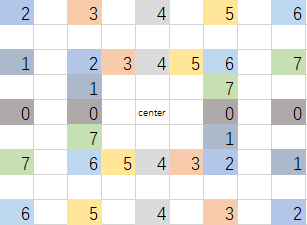
\includegraphics[width=.5\textwidth]{figures/chou.png}
                    \caption{脊线估计方向}\label{adf}
                \end{figure}

            \subsubsection{二值化}
                根据方向场,计算脊线方向$iDir$和法线$iVar = iDir + 4$的灰度平均值$Gmean[iDir]$和$Gmean[iVar]$,二值化:
                \begin{gather*}
                    P(x,y) = \begin{cases}
                        255, & Gmean[iDir] \geqslant Gmean[iVar], \\
                        0, & \text{otherwise}.
                    \end{cases}
                \end{gather*}
                255表示背景和谷线,0表示脊线。预处理效果如图~\ref{zhiwesn}所示:

                \begin{figure}[H]
                    \centering
                    \subfigure[指纹原始图像]{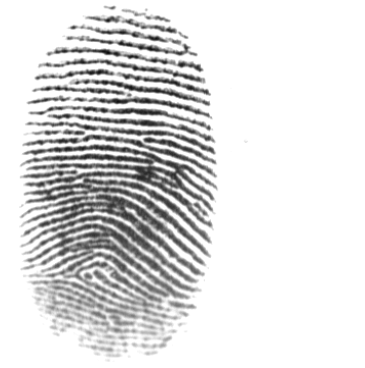
\includegraphics[height=5cm,width=5cm]{figures/rrr.png}}
                    \subfigure[指纹预处理后]{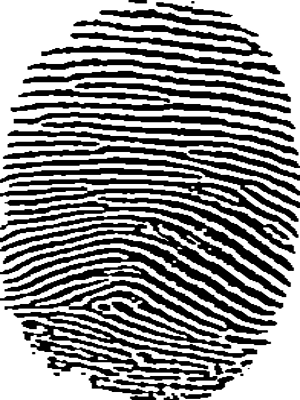
\includegraphics[height=5cm,width=3cm]{figures/result01.png}}
                    \caption{图像预处理效果图}\label{zhiwesn}
                \end{figure}

    % Problem 1: Model establishment and solution
    \section{问题一模型的建立与求解}
        \subsection{问题描述与分析}
            问题一要求用不超过200字节的“指纹密码”描述指纹特征。传统压缩方法(如霍夫曼编码、Golomb编码、LZW编码、小波编码\upcite{7,8,9})在200字节限制下易丢失细节。卷积自编码器通过无监督学习提取关键信息,降低维度,适合小样本编码。

        \subsection{搭建卷积自编码器模型}
            自编码器(AutoEncoder)通过无监督学习生成低维编码,适用于降维和特征检测\upcite{10}。本文基于VGG模型\upcite{4},构造卷积自编码器(CAE),通过交叉验证优化小样本数据参数。

            \subsubsection{卷积神经网络}
                \paragraph{卷积核}
                    矩阵卷积提取图像特征,全卷积定义为:
                    \begin{gather}
                        z(u,v) = \sum_{i=-\infty}^{\infty} \sum_{j=-\infty}^{\infty} x_{i,j} \cdot k_{u-i,v-j},
                    \end{gather}
                    有效值卷积:
                    \begin{gather}
                        z(u,v) = \sum_{i=-\infty}^{\infty} \sum_{j=-\infty}^{\infty} x_{i+u,j+v} \cdot k_{rot,i,j} \cdot \chi(i,j), \quad
                        \chi(i,j) = \begin{cases}
                            1, & 0 \leqslant i,j \leqslant n, \\
                            0, & \text{otherwise}.
                        \end{cases}
                    \end{gather}
                    其中$X$为$m \times m$图像矩阵,$K$为$n \times n$卷积核(通常$3 \times 3$),$K_{rot}$为$K$转置。卷积示意图如图~\ref{cnn}所示:

                    \begin{figure}[H]
                        \centering
                        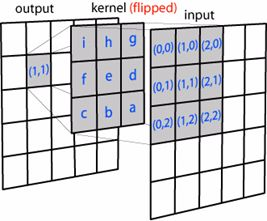
\includegraphics[width=.35\textwidth]{figures/cnn.jpg}
                        \caption{卷积核函数示意图}\label{cnn}
                    \end{figure}

                \paragraph{池化}
                    池化压缩Feature Map,减少参数,增强鲁棒性。Max-Pooling取$2 \times 2$邻域最大值,如图~\ref{pool}所示:

                    \begin{figure}[H]
                        \centering
                        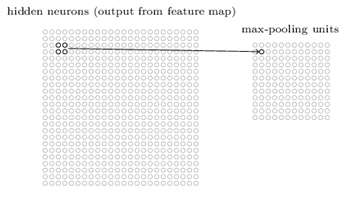
\includegraphics[width=.45\textwidth]{figures/pool.png}
                        \caption{池化层Max-Pooling示意图}\label{pool}
                    \end{figure}

                \paragraph{激活}
                    激活层计算:
                    \begin{gather*}
                        u_k = \sum_{i=1} w_{ki} x_i, \quad y_k = f(u_k - b_k),
                    \end{gather*}
                    使用ReLU激活函数:
                    \begin{gather}
                        f_{\text{ReLU}}(z) = \max(0,z), \quad \frac{d}{dz} f_{\text{ReLU}} = \begin{cases}
                            1, & z > 0, \\
                            0, & z \leqslant 0.
                        \end{cases}
                    \end{gather}
                    输出层使用softmax:
                    \begin{gather}
                        f_{\text{softmax}} = \frac{e^i}{\sum_j e^j}.
                    \end{gather}

            \subsubsection{卷积自编码器}
                给定样本$X = \{x_1, x_2, \dots, x_n\}, X \in \mathbb{R}^{n \times c \times w \times h}$,自编码器编码和解码:
                \begin{gather}
                    \gamma(x) = \text{Encoder}(W_1 x + b), \quad z(x) = \text{Decoder}(W_2 \gamma(x) + c).
                \end{gather}
                最小化重构误差:
                \begin{gather}
                    \theta = \arg \min_\theta L(X,Z) = \arg \min_\theta \frac{1}{2} \sum_{i=1}^N \| x^{(i)} - z(x^{(i)}) \|^2.
                \end{gather}
                CAE编码器结构与CNN卷积池化部分相同,解码器对称,结构如图~\ref{labssel}所示:

                \begin{figure}[H]
                    \centering
                    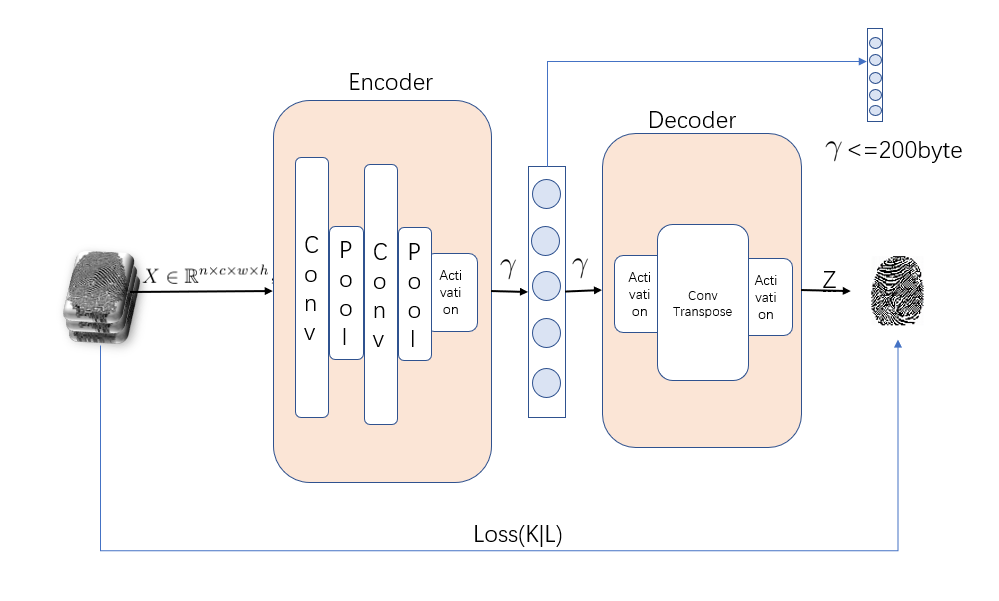
\includegraphics[width=\textwidth]{figures/model.png}
                    \caption{卷积自编码器CAE模型}\label{labssel}
                \end{figure}

                添加稀疏约束,目标函数为:
                \begin{gather}
                    \text{CAE} = L(X,Z) + \gamma \sum_{j=1}^{H_D} \text{KL}(\rho \| \hat{\rho}_j), \\
                    \text{KL}(\rho \| \hat{\rho}_j) = \rho \log \frac{\rho}{\hat{\rho}_j} + (1-\rho) \log \frac{1-\rho}{1-\hat{\rho}_j},
                \end{gather}
                其中$\gamma$为稀疏权重,$H_D$为隐藏单元数,$\rho$为稀疏参数,$\hat{\rho}_j = \frac{1}{N} \sum_{i=1}^N y_j(x^{(i)})$为平均激活。使用Adam优化器:
                \begin{gather}
                    \begin{cases}
                        m_t = \beta_1 m_{t-1} + (1-\beta_1) \nabla_w f(w_t), \\
                        v_t = \beta_2 v_{t-1} + (1-\beta_2) (\nabla_w f(w_t))^2, \\
                        \hat{m}_t = \frac{m_t}{1-\beta_1^t}, \hat{v}_t = \frac{v_t}{1-\beta_2^t}, \\
                        w_t = w_{t-1} - \eta \frac{\hat{m}_t}{\sqrt{\hat{v}_t + \varepsilon}},
                    \end{cases}
                \end{gather}
                其中$\beta_1 = 0.9$,$\beta_2 = 0.999$。

        \subsection{实验结果及分析}
            输入400×300指纹图像,参数设置如表~\ref{param}所示:

            \begin{table}[H]
                \setstretch{1.4}
                \centering
                \caption{参数设置表}
                \label{param}
                \begin{tabular}{cc|cc}
                    \toprule[1.5pt]
                    \multicolumn{1}{m{5cm}}{\centering 参数名称} &
                    \multicolumn{1}{m{2cm}}{\centering 值} &
                    \multicolumn{1}{m{5cm}}{\centering 参数名称} &
                    \multicolumn{1}{m{2cm}}{\centering 值} \\
                    \midrule[1pt]
                    迭代次数 epoch & 2000 & 吞吐量 batch & 64 \\
                    出/入通道数 in/out & 3/3 & 编码大小 size & 200 \\
                    学习率 lr & 0.01 & 偏置 $\beta_1, \beta_2$ & 0.9, 0.999 \\
                    卷积核 $k_1,k_2,k_3$ & 3,3,4 & 池化层 padding & 1 \\
                    \bottomrule[1.5pt]
                \end{tabular}
            \end{table}

            损失函数变化如图~\ref{loss}所示:

            \begin{figure}[H]
                \centering
                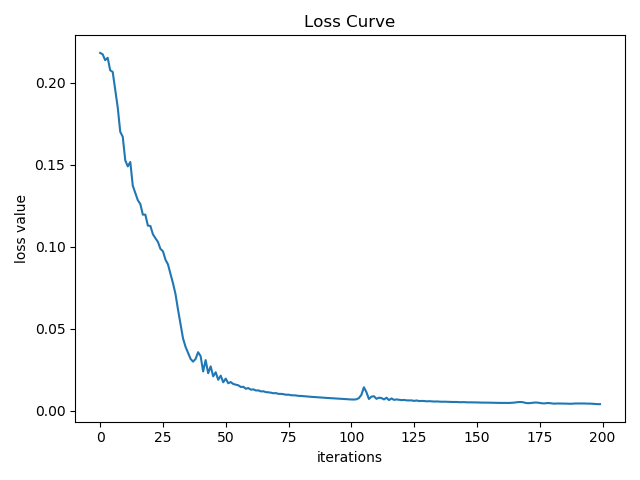
\includegraphics[width=.7\textwidth]{figures/loss.png}
                \caption{CAE迭代过程中损失函数}\label{loss}
            \end{figure}

            信息损失仅0.04\%,优于传统编码。解码图像如图~\ref{zhiwen}所示,迭代超过120次后清晰度接近原始图像。

            \begin{figure}[H]
                \centering
                \subfigure[指纹1解码过程]{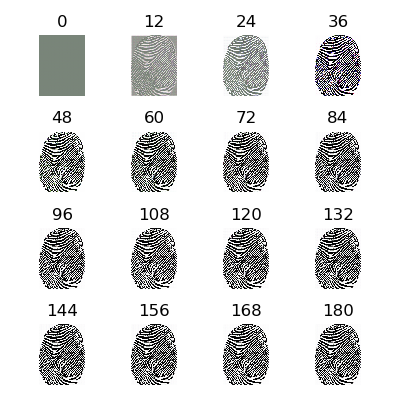
\includegraphics[height=8cm,width=7.5cm]{figures/zhiwen.png}}
                \subfigure[指纹2解码过程]{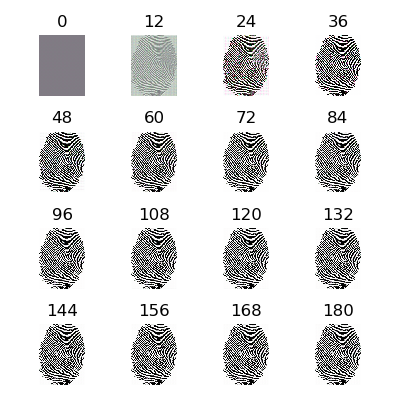
\includegraphics[height=8cm,width=7.5cm]{figures/zhiwen2.png}}
                \caption{解码器还原效果图}\label{zhiwen}
            \end{figure}

        \subsection{灵敏度分析}
            调整编码大小$b$,解码效果如图~\ref{fisg}所示:

            \begin{figure}[H]
                \centering
                \subfigure[$b \leq 10 \text{ byte}$]{
\includegraphics[height=3.5cm,width=3cm]{figures/guo/f1.png}}
                \subfigure[$b \leq 50 \text{ byte}$]{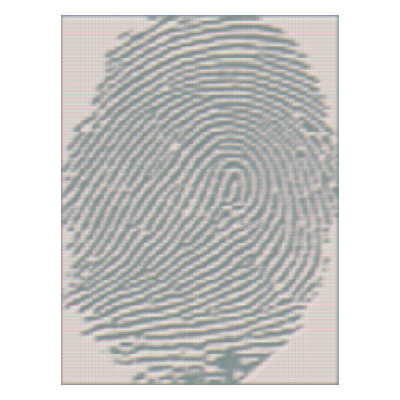
\includegraphics[height=3.5cm,width=3cm]{figures/guo/f2.png}}
                \subfigure[$b \leq 100 \text{ byte}$]{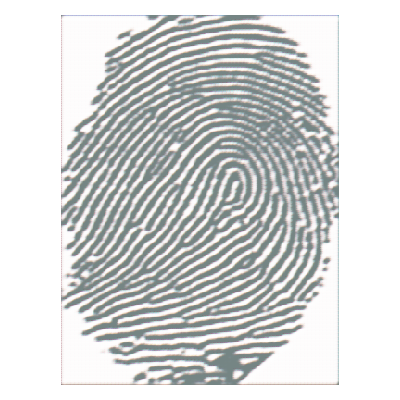
\includegraphics[height=3.5cm,width=3cm]{figures/guo/f3.png}}
                \subfigure[$b \leq 120 \text{ byte}$]{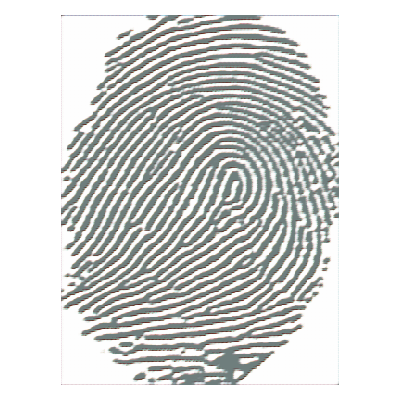
\includegraphics[height=3.5cm,width=3cm]{figures/guo/f4.png}}
                \subfigure[$b \leq 150 \text{ byte}$]{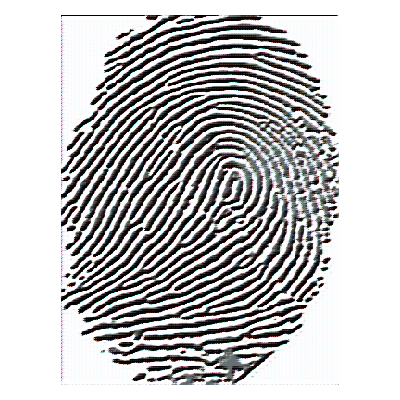
\includegraphics[height=3.5cm,width=3cm]{figures/guo/f5.png}}
                \subfigure[$b \leq 200 \text{ byte}$]{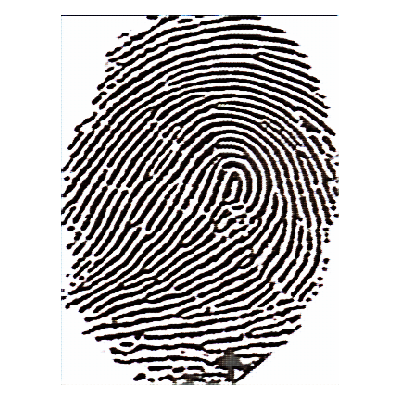
\includegraphics[height=3.5cm,width=3cm]{figures/guo/f6.png}}
                \subfigure[$b \leq 300 \text{ byte}$]{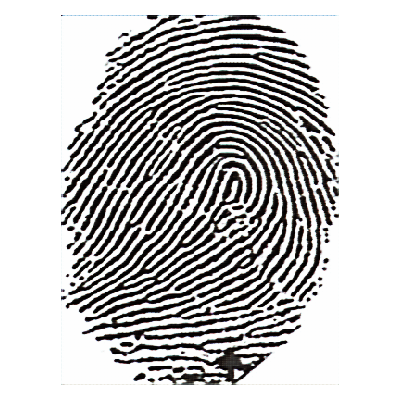
\includegraphics[height=3.5cm,width=3cm]{figures/guo/f7.png}}
                \subfigure[$b \leq 500 \text{ byte}$]{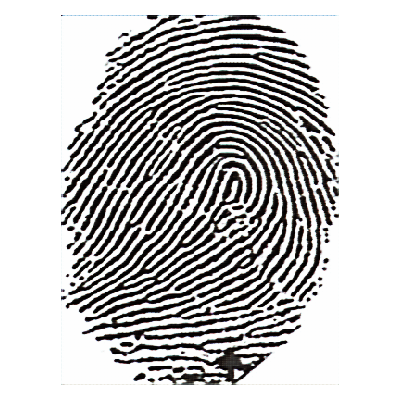
\includegraphics[height=3.5cm,width=3cm]{figures/guo/f8.png}}
                \caption{不同编码字节限制的解码效果}\label{fisg}
            \end{figure}

            50字节可还原大致轮廓,100字节还原微细节但有模糊,150字节较清晰,200字节以上可完美还原。

    % Problem 2: Model establishment and solution
    \section{问题二模型的建立与求解}
        \subsection{问题分析与相似度计算}
            问题二要求基于指纹编码分析相似性。CAE将指纹图像转化为特征向量,相似性分析转化为向量相似度量化。设计加权相似度,归一化向量后计算谷本系数、皮尔逊相关系数和马氏距离,构造关系函数。

            \begin{itemize}
                \item \textbf{谷本系数}
                    用于符号或布尔值相似度:
                    \begin{gather}
                        T(A,B) = \frac{A \cdot B}{\|A\|^2 + \|B\|^2 - A \cdot B}.
                    \end{gather}
                    越大表示相似度越高。
                \item \textbf{皮尔逊相关系数}
                    反映线性相关性:
                    \begin{gather}
                        P(A,B) = \frac{\text{cov}(A,B)}{\sigma_A \cdot \sigma_B},
                    \end{gather}
                    绝对值越大,线性相关性越高。
                \item \textbf{马氏距离}
                    修正欧氏距离:
                    \begin{gather}
                        M(A,B) = \sqrt{(A-B)^T \Sigma^{-1} (A-B)},
                    \end{gather}
                    越小表示相似度越高,$\Sigma$为协方差矩阵。
            \end{itemize}

            相似度函数:
            \begin{gather}
                S(A,B) = \omega_1 T(A,B) + \omega_2 |P(A,B)| + \omega_3 / M(A,B),
            \end{gather}
            其中$\omega_1 + \omega_2 + \omega_3 = 1$,$S(A,B)$越大表示相似度越高。

        \subsection{实验结果及分析}
            取$\omega_1 = 0.2$,$\omega_2 = 0.3$,$\omega_3 = 0.5$,相似度热图如图~\ref{lsst}所示:

            \begin{figure}[H]
                \centering
                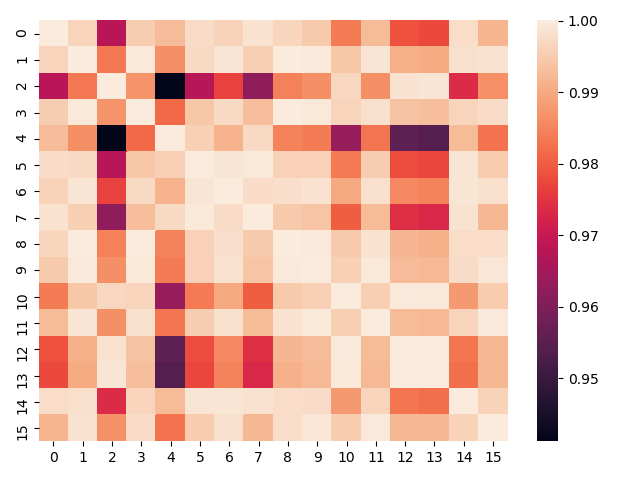
\includegraphics[width=.8\textwidth]{figures/retu.png}
                \caption{距离矩阵相似度热图}\label{lsst}
            \end{figure}

            颜色越浅表示相似度越高,指纹对$\{4,7\}$、$\{1,11\}$、$\{6,13\}$相似度高,$\{4,13\}$、$\{4,2\}$属于不同类型。

        \subsection{灵敏度分析}
            不同权重组合的热图如图~\ref{weight}所示:

            \begin{figure}[H]
                \centering
                \subfigure[$\omega_i = 0.1,0.8,0.1$]{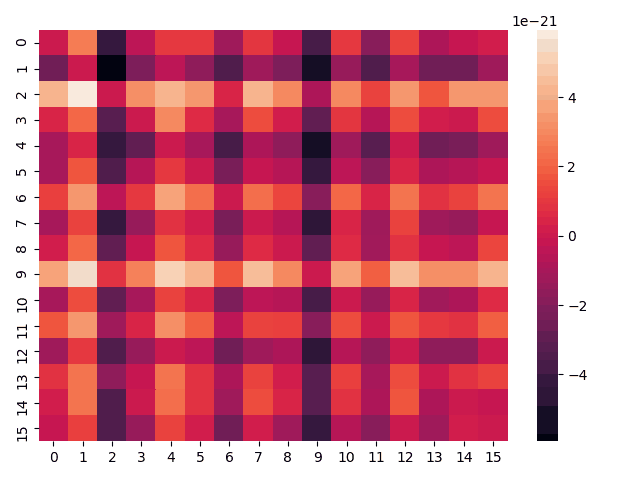
\includegraphics[height=3cm,width=3.5cm]{figures/guo/m1.png}}
                \subfigure[$\omega_i = 0.2,0.5,0.3$]{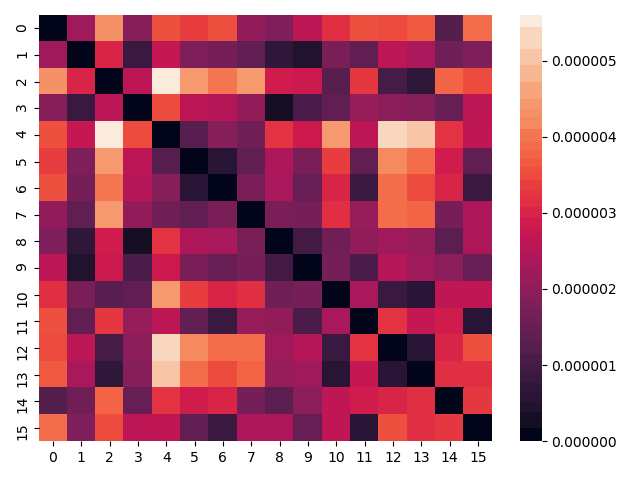
\includegraphics[height=3cm,width=3.5cm]{figures/guo/m2.png}}
                \subfigure[$\omega_i = 0.8,0.1,0.1$]{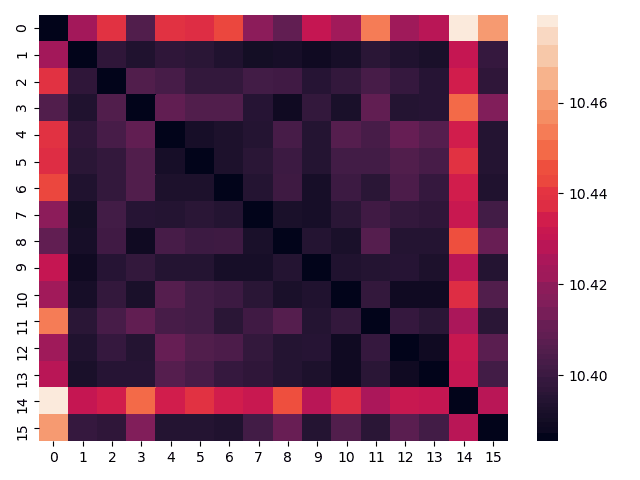
\includegraphics[height=3cm,width=3.5cm]{figures/guo/m3.png}}
                \subfigure[$\omega_i = 0.2,0.3,0.5$]{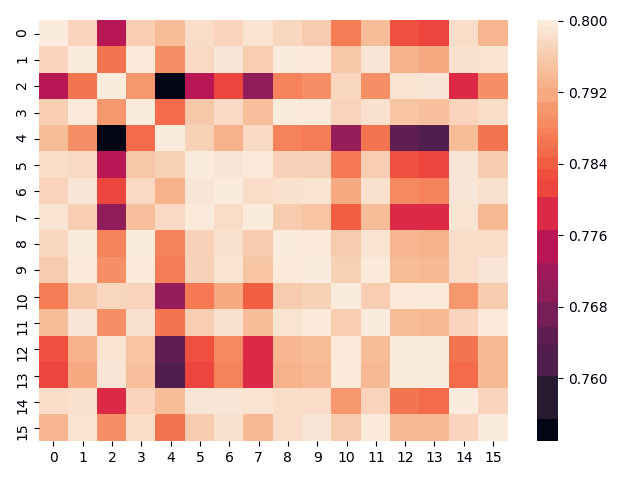
\includegraphics[height=3cm,width=3.5cm]{figures/guo/m4.png}}
                \caption{不同权重分配的相似度热图}\label{weight}
            \end{figure}

            图(d)浅色区域占比适中,深色区域集中,区分度最佳,权重$\omega_1 = 0.2, \omega_2 = 0.3, \omega_3 = 0.5$最优。

    % Problem 3: Model establishment and solution
    \section{问题三模型的建立与求解}
        \subsection{问题描述与分析}
            问题三要求基于问题二的相似度对16个指纹进行分类,属于样本分类问题。加权相似度$S$为非欧氏距离\upcite{10},不适用k-means算法。本文使用k-medoids算法,以相似度平均值为代价函数。

        \subsection{k-medoids模型的建立与求解}
            从16个样本$\{\gamma_i\}$中选$k$个作为聚类中心$\{c_i\}$,代价函数:
            \begin{gather}
                J(c_1, c_2, \dots, c_k) = \frac{1}{16} \sum_{i=1}^{16} \max_{1 \leqslant j \leqslant k} S(\gamma_i, c_j),
            \end{gather}
            优化目标:
            \begin{gather}
                \max \frac{1}{16} \sum_{i=1}^{16} \max_{1 \leqslant j \leqslant k} S(\gamma_i, c_j), \\
                s.t. \ \{ c_j \mid j \in [1,k] \} \subseteq \{ \gamma_i \mid i \in [1,16] \}.
            \end{gather}
            样本规模小,采用遍历搜索最优聚类中心,伪代码如下:

            \begin{algorithm}[H]
                \caption{k-medoids算法}
                \setstretch{0.8}
                \LinesNumbered
                \KwIn{聚类中心数: $k$}
                \KwOut{聚类中心: $\{c_i\}$}
                \textbf{Initialize} $J_{\max} \leftarrow 0$ \\
                \For{$\pi_1 = 1$ to $16-k+1$}{
                    \For{$\pi_2 = \pi_1+1$ to $16-k+2$}{
                        $\vdots$ \\
                        \For{$\pi_k = \pi_{k-1}+1$ to $16$}{
                            \If{$J(\gamma_{\pi_1}, \gamma_{\pi_2}, \dots, \gamma_{\pi_k}) > J_{\max}$}{
                                $J_{\max} = J(\gamma_{\pi_1}, \gamma_{\pi_2}, \dots, \gamma_{\pi_k})$ \\
                                $\{c_i\} = \{\gamma_{\pi_1}, \gamma_{\pi_2}, \dots, \gamma_{\pi_k}\}$
                            }
                        }
                        $\vdots$
                    }
                }
                \Return{$\{c_i\}$}
            \end{algorithm}

        \subsection{实验结果及分析}
            聚类树状图如图~\ref{bgbgbg}所示:

            \begin{figure}[H]
                \centering
                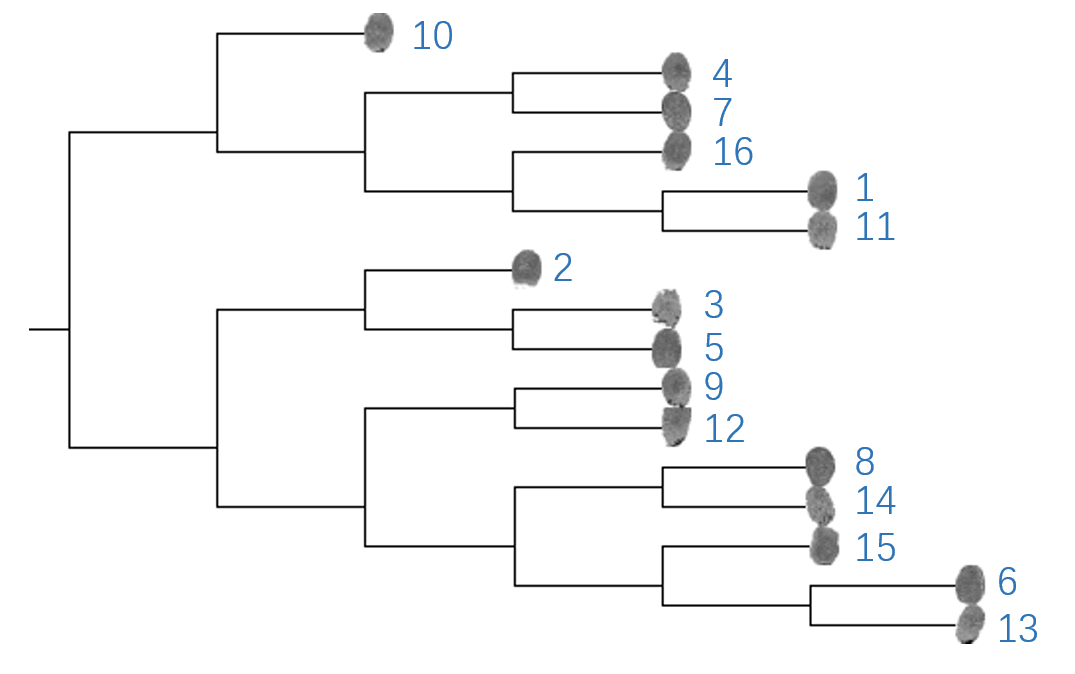
\includegraphics[width=.8\textwidth]{figures/tree.png}
                \caption{指纹聚类树状图}\label{bgbgbg}
            \end{figure}

            当$k=2$,分为$\{1,4,7,10,11,16\}$和$\{2,3,5,6,8,9,12,13,14,15\}$;当$k=4$,样本10独立,其余为$\{2,3,5\}$、$\{1,4,7,11,16\}$和$\{6,8,9,12,13,14,15\}$。$k=4$时代价函数最优,分类如图~\ref{bgssssbgbg}所示,命名为螺形纹、环形纹、弓形纹、箕形纹。

            \begin{figure}[H]
                \centering
                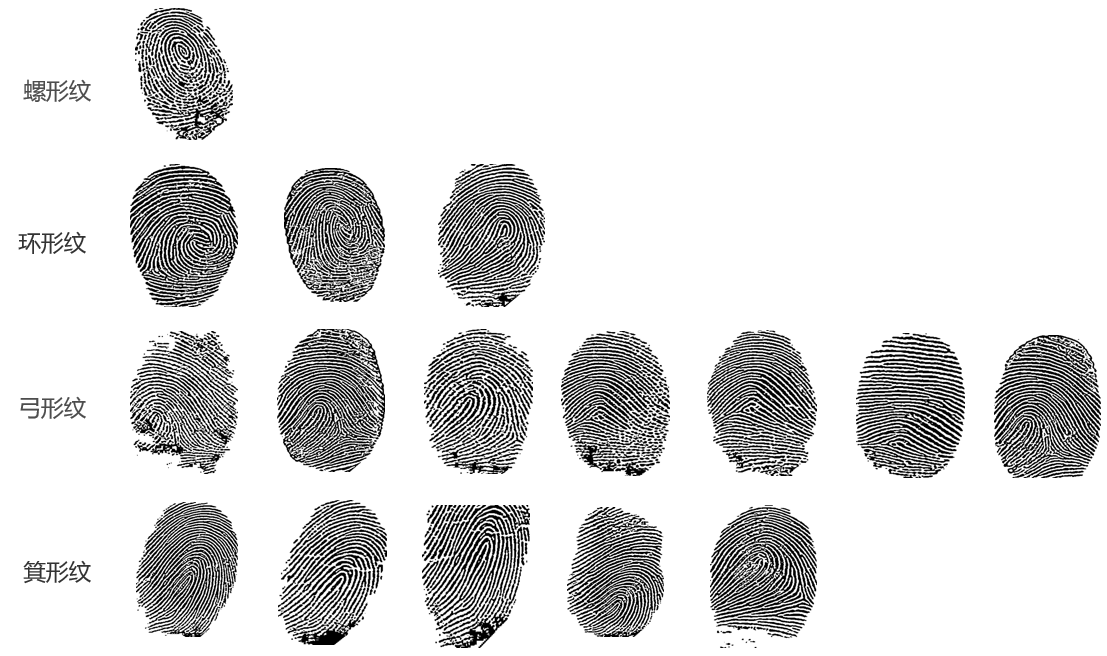
\includegraphics[width=.8\textwidth]{figures/gg.png}
                \caption{指纹图像的识别与分类}\label{bgssssbgbg}
            \end{figure}

    % Model evaluation
    \section{模型的评价}
        \subsection{模型的优点}
            \begin{itemize}
                \item[(1)] 卷积核通过无监督学习提取指纹细节,压缩数据,保留关键信息。
                \item[(2)] CAE在小样本条件下超越传统编码,可高精度还原图像。
            \end{itemize}

        \subsection{模型的缺点}
            小样本数据易导致过拟合,需更多样本训练。

        \subsection{模型总结与展望}
            CAE可优化Encoder-Decoder结构。Lucas Theis等人\upcite{16}提出由ComCNN和RecCNN组成的压缩网络,ComCNN提取紧凑表示,RecCNN进行超分辨率重建。有损自编码器可结合概率模型Q分配熵编码比特数\upcite{17,18},在高斯尺度混合中优化低比特率失真。

    % References
    \newpage
    \nocite{*}
    \begin{thebibliography}{9}
        \bibitem{1} Davies S G. Touching Big Brother: How biometric technology will fuse flesh and machine[J]. Information Technology \& People, 2014, 7(4): 38-47.
        \bibitem{2} Moses K R, Higgins P, McCabe M, et al. Automated fingerprint identification system (AFIS)[J]. Scientific Working Group on Friction Ridge Analysis Study and Technology and National institute of Justice (eds.) SWGFAST-The fingerprint sourcebook, 2011: 1-33.
        \bibitem{3} Dror I E, Wertheim K, Fraser‐Mackenzie P, et al. The impact of human–technology cooperation and distributed cognition in forensic science: biasing effects of AFIS contextual information on human experts[J]. Journal of forensic sciences, 2012, 57(2): 343-352.
        \bibitem{4} Simonyan K, Zisserman A. Very deep convolutional networks for large-scale image recognition[J]. arXiv preprint arXiv:1409.1556, 2014.
        \bibitem{5} Scherer R, Kalla S L, Tang Y, et al. The Grünwald–Letnikov method for fractional differential equations[J]. Computers \& Mathematics with Applications, 2011, 62(3): 902-917.
        \bibitem{6} 邓正宏, 丁有军. 基于动态方向场的指纹图像增强算法[J]. 微电子学与计算机, 2005, 22(2): 70-72.
        \bibitem{7} 蓝波, 林小竹, 籍俊伟. 一种改进的 LZW 算法在图像编码中的应用[J]. 计算机工程与科学, 2006, 28(6): 55-57.
        \bibitem{8} 张旭东. 图像编码基础和小波压缩技术: 原理, 算法和标准[M]. 清华大学出版社有限公司, 2004.
        \bibitem{9} 赵利平, 林涛, 周开伦. 屏幕图像压缩中串复制位移参数的高效编码算法[J]. 计算机学报, 2017, 40(5): 1218-1228.
        \bibitem{10} 黄健航, 雷迎科. 基于边际 Fisher 深度自编码器的电台指纹特征提取[J]. 模式识别与人工智能, 2017 (2017 年 11): 1030-1038.
        \bibitem{11} Gao L, Chen P Y, Yu S. Demonstration of convolution kernel operation on resistive cross-point array[J]. IEEE Electron Device Letters, 2016, 37(7): 870-873.
        \bibitem{12} Guo X, Liu X, Zhu E, et al. Deep clustering with convolutional autoencoders[C]//International conference on neural information processing. Springer, Cham, 2017: 373-382.
        \bibitem{13} 王万良, 杨小涵, 赵燕伟, 等. 采用卷积自编码器网络的图像增强算法[J]. 浙江大学学报 (工学版), 2019, 53(9): 1728-1740.
        \bibitem{14} Arora P, Varshney S. Analysis of k-means and k-medoids algorithm for big data[J]. Procedia Computer Science, 2016, 78: 507-512.
        \bibitem{15} Yu D, Liu G, Guo M, et al. An improved K-medoids algorithm based on step increasing and optimizing medoids[J]. Expert Systems with Applications, 2018, 92: 464-473.
        \bibitem{16} Theis L, Shi W, Cunningham A, et al. Lossy image compression with compressive autoencoders[J]. arXiv preprint arXiv:1703.00395, 2017.
        \bibitem{17} Huszar F, Theis L, Shi W, et al. Lossy Image Compression with Compressive Autoencoders[J]. 2020.
        \bibitem{18} Mukherjee R, Chandran S. Lossy image compression using SVD coding, compressive autoencoders, and prediction error-vector quantization[C]//2017 4th International Conference on Opto-Electronics and Applied Optics (Optronix). IEEE, 2017: 1-5.
    \end{thebibliography}

    % Appendix
    \newpage
    \appendix
    % \section{数据预处理}
        % \subsection*{去噪--MATLAB源代码}
            % \lstinputlisting[language=matlab]{./code/denoise.m}
        % \subsection*{图像处理--MATLAB源代码}
            % \lstinputlisting[language=matlab]{./code/process_image.m}
    \section{第一问代码实现及可视化}
        \subsection*{卷积自编码器--Python源代码}
            \lstinputlisting[language=python]{./code/tuxiang.py}
    \section{第二、三问代码实现及可视化}
        \subsection*{k-medoids模型--Python源代码}
            \lstinputlisting[language=python]{./code/julei.py}
\end{document}